% Options for packages loaded elsewhere
% Options for packages loaded elsewhere
\PassOptionsToPackage{unicode}{hyperref}
\PassOptionsToPackage{hyphens}{url}
\PassOptionsToPackage{dvipsnames,svgnames,x11names}{xcolor}
%
\documentclass[
  letterpaper,
  DIV=11,
  numbers=noendperiod]{scrartcl}
\usepackage{xcolor}
\usepackage{amsmath,amssymb}
\setcounter{secnumdepth}{5}
\usepackage{iftex}
\ifPDFTeX
  \usepackage[T1]{fontenc}
  \usepackage[utf8]{inputenc}
  \usepackage{textcomp} % provide euro and other symbols
\else % if luatex or xetex
  \usepackage{unicode-math} % this also loads fontspec
  \defaultfontfeatures{Scale=MatchLowercase}
  \defaultfontfeatures[\rmfamily]{Ligatures=TeX,Scale=1}
\fi
\usepackage{lmodern}
\ifPDFTeX\else
  % xetex/luatex font selection
\fi
% Use upquote if available, for straight quotes in verbatim environments
\IfFileExists{upquote.sty}{\usepackage{upquote}}{}
\IfFileExists{microtype.sty}{% use microtype if available
  \usepackage[]{microtype}
  \UseMicrotypeSet[protrusion]{basicmath} % disable protrusion for tt fonts
}{}
\makeatletter
\@ifundefined{KOMAClassName}{% if non-KOMA class
  \IfFileExists{parskip.sty}{%
    \usepackage{parskip}
  }{% else
    \setlength{\parindent}{0pt}
    \setlength{\parskip}{6pt plus 2pt minus 1pt}}
}{% if KOMA class
  \KOMAoptions{parskip=half}}
\makeatother
% Make \paragraph and \subparagraph free-standing
\makeatletter
\ifx\paragraph\undefined\else
  \let\oldparagraph\paragraph
  \renewcommand{\paragraph}{
    \@ifstar
      \xxxParagraphStar
      \xxxParagraphNoStar
  }
  \newcommand{\xxxParagraphStar}[1]{\oldparagraph*{#1}\mbox{}}
  \newcommand{\xxxParagraphNoStar}[1]{\oldparagraph{#1}\mbox{}}
\fi
\ifx\subparagraph\undefined\else
  \let\oldsubparagraph\subparagraph
  \renewcommand{\subparagraph}{
    \@ifstar
      \xxxSubParagraphStar
      \xxxSubParagraphNoStar
  }
  \newcommand{\xxxSubParagraphStar}[1]{\oldsubparagraph*{#1}\mbox{}}
  \newcommand{\xxxSubParagraphNoStar}[1]{\oldsubparagraph{#1}\mbox{}}
\fi
\makeatother

\usepackage{color}
\usepackage{fancyvrb}
\newcommand{\VerbBar}{|}
\newcommand{\VERB}{\Verb[commandchars=\\\{\}]}
\DefineVerbatimEnvironment{Highlighting}{Verbatim}{commandchars=\\\{\}}
% Add ',fontsize=\small' for more characters per line
\usepackage{framed}
\definecolor{shadecolor}{RGB}{241,243,245}
\newenvironment{Shaded}{\begin{snugshade}}{\end{snugshade}}
\newcommand{\AlertTok}[1]{\textcolor[rgb]{0.68,0.00,0.00}{#1}}
\newcommand{\AnnotationTok}[1]{\textcolor[rgb]{0.37,0.37,0.37}{#1}}
\newcommand{\AttributeTok}[1]{\textcolor[rgb]{0.40,0.45,0.13}{#1}}
\newcommand{\BaseNTok}[1]{\textcolor[rgb]{0.68,0.00,0.00}{#1}}
\newcommand{\BuiltInTok}[1]{\textcolor[rgb]{0.00,0.23,0.31}{#1}}
\newcommand{\CharTok}[1]{\textcolor[rgb]{0.13,0.47,0.30}{#1}}
\newcommand{\CommentTok}[1]{\textcolor[rgb]{0.37,0.37,0.37}{#1}}
\newcommand{\CommentVarTok}[1]{\textcolor[rgb]{0.37,0.37,0.37}{\textit{#1}}}
\newcommand{\ConstantTok}[1]{\textcolor[rgb]{0.56,0.35,0.01}{#1}}
\newcommand{\ControlFlowTok}[1]{\textcolor[rgb]{0.00,0.23,0.31}{\textbf{#1}}}
\newcommand{\DataTypeTok}[1]{\textcolor[rgb]{0.68,0.00,0.00}{#1}}
\newcommand{\DecValTok}[1]{\textcolor[rgb]{0.68,0.00,0.00}{#1}}
\newcommand{\DocumentationTok}[1]{\textcolor[rgb]{0.37,0.37,0.37}{\textit{#1}}}
\newcommand{\ErrorTok}[1]{\textcolor[rgb]{0.68,0.00,0.00}{#1}}
\newcommand{\ExtensionTok}[1]{\textcolor[rgb]{0.00,0.23,0.31}{#1}}
\newcommand{\FloatTok}[1]{\textcolor[rgb]{0.68,0.00,0.00}{#1}}
\newcommand{\FunctionTok}[1]{\textcolor[rgb]{0.28,0.35,0.67}{#1}}
\newcommand{\ImportTok}[1]{\textcolor[rgb]{0.00,0.46,0.62}{#1}}
\newcommand{\InformationTok}[1]{\textcolor[rgb]{0.37,0.37,0.37}{#1}}
\newcommand{\KeywordTok}[1]{\textcolor[rgb]{0.00,0.23,0.31}{\textbf{#1}}}
\newcommand{\NormalTok}[1]{\textcolor[rgb]{0.00,0.23,0.31}{#1}}
\newcommand{\OperatorTok}[1]{\textcolor[rgb]{0.37,0.37,0.37}{#1}}
\newcommand{\OtherTok}[1]{\textcolor[rgb]{0.00,0.23,0.31}{#1}}
\newcommand{\PreprocessorTok}[1]{\textcolor[rgb]{0.68,0.00,0.00}{#1}}
\newcommand{\RegionMarkerTok}[1]{\textcolor[rgb]{0.00,0.23,0.31}{#1}}
\newcommand{\SpecialCharTok}[1]{\textcolor[rgb]{0.37,0.37,0.37}{#1}}
\newcommand{\SpecialStringTok}[1]{\textcolor[rgb]{0.13,0.47,0.30}{#1}}
\newcommand{\StringTok}[1]{\textcolor[rgb]{0.13,0.47,0.30}{#1}}
\newcommand{\VariableTok}[1]{\textcolor[rgb]{0.07,0.07,0.07}{#1}}
\newcommand{\VerbatimStringTok}[1]{\textcolor[rgb]{0.13,0.47,0.30}{#1}}
\newcommand{\WarningTok}[1]{\textcolor[rgb]{0.37,0.37,0.37}{\textit{#1}}}

\usepackage{longtable,booktabs,array}
\usepackage{calc} % for calculating minipage widths
% Correct order of tables after \paragraph or \subparagraph
\usepackage{etoolbox}
\makeatletter
\patchcmd\longtable{\par}{\if@noskipsec\mbox{}\fi\par}{}{}
\makeatother
% Allow footnotes in longtable head/foot
\IfFileExists{footnotehyper.sty}{\usepackage{footnotehyper}}{\usepackage{footnote}}
\makesavenoteenv{longtable}
\usepackage{graphicx}
\makeatletter
\newsavebox\pandoc@box
\newcommand*\pandocbounded[1]{% scales image to fit in text height/width
  \sbox\pandoc@box{#1}%
  \Gscale@div\@tempa{\textheight}{\dimexpr\ht\pandoc@box+\dp\pandoc@box\relax}%
  \Gscale@div\@tempb{\linewidth}{\wd\pandoc@box}%
  \ifdim\@tempb\p@<\@tempa\p@\let\@tempa\@tempb\fi% select the smaller of both
  \ifdim\@tempa\p@<\p@\scalebox{\@tempa}{\usebox\pandoc@box}%
  \else\usebox{\pandoc@box}%
  \fi%
}
% Set default figure placement to htbp
\def\fps@figure{htbp}
\makeatother


% definitions for citeproc citations
\NewDocumentCommand\citeproctext{}{}
\NewDocumentCommand\citeproc{mm}{%
  \begingroup\def\citeproctext{#2}\cite{#1}\endgroup}
\makeatletter
 % allow citations to break across lines
 \let\@cite@ofmt\@firstofone
 % avoid brackets around text for \cite:
 \def\@biblabel#1{}
 \def\@cite#1#2{{#1\if@tempswa , #2\fi}}
\makeatother
\newlength{\cslhangindent}
\setlength{\cslhangindent}{1.5em}
\newlength{\csllabelwidth}
\setlength{\csllabelwidth}{3em}
\newenvironment{CSLReferences}[2] % #1 hanging-indent, #2 entry-spacing
 {\begin{list}{}{%
  \setlength{\itemindent}{0pt}
  \setlength{\leftmargin}{0pt}
  \setlength{\parsep}{0pt}
  % turn on hanging indent if param 1 is 1
  \ifodd #1
   \setlength{\leftmargin}{\cslhangindent}
   \setlength{\itemindent}{-1\cslhangindent}
  \fi
  % set entry spacing
  \setlength{\itemsep}{#2\baselineskip}}}
 {\end{list}}
\usepackage{calc}
\newcommand{\CSLBlock}[1]{\hfill\break\parbox[t]{\linewidth}{\strut\ignorespaces#1\strut}}
\newcommand{\CSLLeftMargin}[1]{\parbox[t]{\csllabelwidth}{\strut#1\strut}}
\newcommand{\CSLRightInline}[1]{\parbox[t]{\linewidth - \csllabelwidth}{\strut#1\strut}}
\newcommand{\CSLIndent}[1]{\hspace{\cslhangindent}#1}



\setlength{\emergencystretch}{3em} % prevent overfull lines

\providecommand{\tightlist}{%
  \setlength{\itemsep}{0pt}\setlength{\parskip}{0pt}}



 


\usepackage{booktabs}
\usepackage{caption}
\usepackage{longtable}
\usepackage{colortbl}
\usepackage{array}
\usepackage{anyfontsize}
\usepackage{multirow}
\KOMAoption{captions}{tableheading}
\usepackage{float}
\makeatletter
\@ifpackageloaded{caption}{}{\usepackage{caption}}
\AtBeginDocument{%
\ifdefined\contentsname
  \renewcommand*\contentsname{Table of contents}
\else
  \newcommand\contentsname{Table of contents}
\fi
\ifdefined\listfigurename
  \renewcommand*\listfigurename{List of Figures}
\else
  \newcommand\listfigurename{List of Figures}
\fi
\ifdefined\listtablename
  \renewcommand*\listtablename{List of Tables}
\else
  \newcommand\listtablename{List of Tables}
\fi
\ifdefined\figurename
  \renewcommand*\figurename{Figure}
\else
  \newcommand\figurename{Figure}
\fi
\ifdefined\tablename
  \renewcommand*\tablename{Table}
\else
  \newcommand\tablename{Table}
\fi
}
\@ifpackageloaded{float}{}{\usepackage{float}}
\floatstyle{ruled}
\@ifundefined{c@chapter}{\newfloat{codelisting}{h}{lop}}{\newfloat{codelisting}{h}{lop}[chapter]}
\floatname{codelisting}{Listing}
\newcommand*\listoflistings{\listof{codelisting}{List of Listings}}
\makeatother
\makeatletter
\makeatother
\makeatletter
\@ifpackageloaded{caption}{}{\usepackage{caption}}
\@ifpackageloaded{subcaption}{}{\usepackage{subcaption}}
\makeatother
\usepackage{bookmark}
\IfFileExists{xurl.sty}{\usepackage{xurl}}{} % add URL line breaks if available
\urlstyle{same}
\hypersetup{
  pdftitle={int3ract: Johnson--Neyman Technique and Its Three-Way Extension for Frequentist and Bayesian Models in R},
  pdfauthor={Robert W. Krause},
  pdfkeywords={interaction effects, Johnson-Neyman technique, moderation
analysis, SAOM, Bayesian, R},
  colorlinks=true,
  linkcolor={blue},
  filecolor={Maroon},
  citecolor={Blue},
  urlcolor={Blue},
  pdfcreator={LaTeX via pandoc}}


\title{\textbf{int3ract}: Johnson--Neyman Technique and Its Three-Way
Extension for Frequentist and Bayesian Models in R}
\author{Robert W. Krause}
\date{}
\begin{document}
\maketitle
\begin{abstract}
Interaction effects are ubiquitous in applied statistical modelling, yet
their meaningful interpretation remains challenging. The classic
Johnson--Neyman (JN) technique (Johnson and Neyman 1936) addresses this
challenge for two-way interactions by identifying the regions of a
moderator's range over which a focal effect is and is not statistically
significant. The \textbf{int3ract} package for R implements the JN
technique and its three-way extension (the Johnson--Neyman--Krause, or
JNK, technique) for both frequentist and Bayesian models. The core
function \texttt{freq\_int()} can be applied to multiplicative
interactions from (virtually) any model family. Dedicated wrappers
(\texttt{JNK\_lm()} and \texttt{JNK\_siena()}) streamline the workflow
for models fitted via \texttt{lm()}/\texttt{glm()} and \textbf{RSiena}'s
\texttt{siena()}, respectively. For Bayesian Stochastic Actor-Oriented
Models (SAOMs) estimated with \textbf{multiSiena}, the function
\texttt{JNSienaBayes()} produces conditional posterior distributions.
For two-way interactions, classic shaded confidence-band plots are
created that visually demarcate significant and non-significant regions
along the moderator range; three-way interactions yield colour-gradient
heatmaps with optional crosshatch overlays for non-significant regions.
The package is designed to encourage richer, region-specific reporting
of interaction effects in place of the conventional single-slope
spotlight approach.
\end{abstract}


\section{Introduction}\label{sec-intro}

Multiplicative interaction terms allow researchers to examine whether
the relationship between a predictor \(X\) and an outcome \(Y\) depends
on the value of one or more additional variables---the so-called
moderators. Interpreting such interactions by inspecting the sign and
significance of the interaction coefficient alone is, however,
insufficient and potentially misleading (Bauer and Curran 2005;
Preacher, Curran, and Bauer 2006). The key insight behind the
Johnson--Neyman (JN) technique is that instead of evaluating the focal
effect at a small number of selected moderator values (often referred to
as ``spotlight'' or ``simple-slope''), one can derive the \emph{entire}
region of the moderator's distribution over which the focal effect is
statistically distinguishable from zero (Johnson and Neyman 1936;
Potthoff 1964).

Originally proposed in the context of the analysis of covariance
(Johnson and Neyman 1936), the JN technique was later adapted for
regression (Potthoff 1964) and updated by Bauer and Curran (2005), whose
formulation is closest to what \textbf{int3ract} implements. Several R
packages already address the two-way JN case, for instance,
\textbf{interactions} (Long 2019) and \textbf{jtools} (Long 2020). The
contribution of \textbf{int3ract} is threefold.

\begin{enumerate}
\def\labelenumi{\arabic{enumi}.}
\item
  \textbf{Three-way interactions.} The package provides a complete
  implementation of the JNK technique for three-way multiplicative
  interactions, producing a heatmap over the two-dimensional moderator
  grid rather than a single-axis ribbon plot.
\item
  \textbf{Model-agnostic frequentist engine.} The internal function
  \texttt{freq\_int()} requires only a coefficient vector and the
  relevant sub-matrix of the parameter covariance matrix. It therefore
  applies to any frequentist model that produces these
  quantities---ordinary least squares, generalised linear models,
  mixed-effects models, survival models, or Stochastic Actor-Oriented
  Models---without modification.
\item
  \textbf{Bayesian SAOMs.} The function \texttt{JNSienaBayes()} adapts
  the technique to the posterior distribution rather than the sampling
  distribution, producing density plots (two-way) and posterior-mean
  heatmaps with Bayesian \(p\)-value overlays (three-way) for models
  estimated with \textbf{multiSiena}.
\end{enumerate}

The remainder of the paper is organised as follows.
Section~\ref{sec-background} reviews the statistical background of the
JN technique and its three-way extension. Section~\ref{sec-package}
describes the package architecture. Section~\ref{sec-freq} and
Section~\ref{sec-bayes} illustrate the frequentist and Bayesian
workflows with worked examples. Section~\ref{sec-graphics} discusses
graphical customisation. Section~\ref{sec-conc} concludes.

\section{Statistical Background}\label{sec-background}

\subsection{The Two-Way Johnson--Neyman
Technique}\label{the-two-way-johnsonneyman-technique}

Consider the linear model

\begin{equation}\phantomsection\label{eq-2way}{
Y_i = \beta_0 + \beta_1 X_i + \beta_2 M_i + \beta_3 X_i M_i + \varepsilon_i,
}\end{equation}

where \(X\) is the focal predictor, \(M\) is the moderator, and
\(\beta_3\) is the interaction coefficient. The simple slope of \(Y\)
with respect to \(X\) at a given value \(m\) of the moderator is

\begin{equation}\phantomsection\label{eq-simpleslope}{
\hat{\theta}_X(m) = \hat{\beta}_1 + \hat{\beta}_3 \, m.
}\end{equation}

Its sampling variance follows from the delta method:

\begin{equation}\phantomsection\label{eq-var2way}{
\widehat{Var}\bigl[\hat{\theta}_X(m)\bigr]
  = \widehat{Var}(\hat{\beta}_1)
    + 2m\,\widehat{Cov}(\hat{\beta}_1, \hat{\beta}_3)
    + m^2\,\widehat{Var}(\hat{\beta}_3).
}\end{equation}

The two-way JN regions are the set of moderator values \(m\) for which
the two-sided \(z\)-test

\[
z(m) = \frac{\hat{\theta}_X(m)}
            {\sqrt{\widehat{Var}[\hat{\theta}_X(m)]}}
\]

satisfies \(|z(m)| > z_{\alpha/2}\), where \(z_{\alpha/2}\) is the
\((\alpha/2)\)-upper quantile of the standard normal distribution.

The symmetry of Equation~\ref{eq-2way} implies that the roles of \(X\)
and \(M\) are interchangeable: the simple slope of \(Y\) on \(M\)
moderated by \(X\) is \(\hat{\beta}_2 + \hat{\beta}_3 \, x\), with an
analogous variance formula. \textbf{int3ract} therefore always produces
\emph{two} JN plots per two-way interaction and three for three-way
interactions -- one for each variable acting as the focal predictor.

\subsection{The Three-Way Extension}\label{sec-threeway}

When a third variable \(W\) enters as an additional moderator, the full
three-way interaction model is

\begin{equation}\phantomsection\label{eq-3way}{
\begin{aligned}
Y_i = \; & \beta_0 + \beta_1 X_i + \beta_2 M_i + \beta_3 W_i
           + \beta_4 X_i M_i + \beta_5 X_i W_i + \beta_6 M_i W_i \\
         & + \beta_7 X_i M_i W_i + \varepsilon_i.
\end{aligned}
}\end{equation}

The conditional effect of \(X\) given \(M\) and \(W\) is

\begin{equation}\phantomsection\label{eq-theta3way}{
\theta_X(m, w)
  = \beta_1 + \beta_4 m + \beta_5 w + \beta_7 mw,
}\end{equation}

and the corresponding standard error is obtained via the multivariate
delta method:

\begin{equation}\phantomsection\label{eq-se3way}{
\begin{aligned}
\widehat{Var}\bigl[\hat{\theta}_X(m,w)\bigr]
  = \; & \widehat{Var}_{\beta_1}
      + m^2 \widehat{Var}_{\beta_4}
      + w^2 \widehat{Var}_{\beta_5}
      + (m w)^2 \widehat{Var}_{\beta_7} \\
    & + 2m \widehat{Cov}(\beta_1,\beta_4)
      + 2w \widehat{Cov}(\beta_1,\beta_5)
      + 2m w \widehat{Cov}(\beta_1,\beta_7) \\
    & + 2m w \widehat{Cov}(\beta_4,\beta_5)
      + 2m^2 w \widehat{Cov}(\beta_4,\beta_7) \\
    & + 2m w^2 \widehat{Cov}(\beta_5,\beta_7).
\end{aligned}
}\end{equation}

Because the significance region is now two-dimensional, it cannot be
depicted as a simple interval on a line. \textbf{int3ract} instead
renders a heatmap of conditional point estimates
\(\hat{\theta}_X(m, w)\) using a diverging colour scale, and
superimposes a crosshatch pattern over cells where the null hypothesis
\(\theta_X = 0\) should be rejected given the chosen
\(\alpha\)-threshold (default: \texttt{threshold\ =\ 0.05}).

\section{Package Architecture}\label{sec-package}

The package is organised into four layers, summarised in
Table~\ref{tbl-hierarchy}.

\begin{longtable}[]{@{}
  >{\raggedright\arraybackslash}p{(\linewidth - 4\tabcolsep) * \real{0.3333}}
  >{\raggedright\arraybackslash}p{(\linewidth - 4\tabcolsep) * \real{0.3333}}
  >{\raggedright\arraybackslash}p{(\linewidth - 4\tabcolsep) * \real{0.3333}}@{}}
\caption{Function hierarchy of \textbf{int3ract}. User-facing wrappers
extract the relevant coefficients and covariance sub-matrix from the
model object and pass them to the appropriate
engine.}\label{tbl-hierarchy}\tabularnewline
\toprule\noalign{}
\begin{minipage}[b]{\linewidth}\raggedright
Entry point
\end{minipage} & \begin{minipage}[b]{\linewidth}\raggedright
Model class
\end{minipage} & \begin{minipage}[b]{\linewidth}\raggedright
Core engine
\end{minipage} \\
\midrule\noalign{}
\endfirsthead
\toprule\noalign{}
\begin{minipage}[b]{\linewidth}\raggedright
Entry point
\end{minipage} & \begin{minipage}[b]{\linewidth}\raggedright
Model class
\end{minipage} & \begin{minipage}[b]{\linewidth}\raggedright
Core engine
\end{minipage} \\
\midrule\noalign{}
\endhead
\bottomrule\noalign{}
\endlastfoot
\texttt{JNK\_lm()} & \texttt{lm}, \texttt{glm} & \texttt{freq\_int()} \\
\texttt{JNK\_siena()} & \texttt{sienaFit} (frequentist) &
\texttt{freq\_int()} \\
\texttt{JNSienaBayes()} & \texttt{multiSiena} (Bayesian) &
\texttt{jnb\_support2()}, \texttt{jnb\_support3()} \\
\texttt{freq\_int()} & \emph{any} (generic) & \texttt{parFun()},
\texttt{seFun()} \\
\end{longtable}

\textbf{Utility layer (\texttt{utils.R}).}\\
\texttt{parFun()} and \texttt{seFun()} implement
Equation~\ref{eq-theta3way} and Equation~\ref{eq-se3way}.

\textbf{Core frequentist engine (\texttt{freq\_int()}).}\\
The function \texttt{freq\_int()} accepts \texttt{name} (character
vector of variable names), \texttt{coefs} (named numeric vector of model
coefficients), \texttt{covar} (the corresponding covariance sub-matrix),
and \texttt{vals} (a list of moderator value ranges). When a 2-way
interaction is analysed, it returns two ribbon plots and two data
frames; when a 3-way interaction, it returns three heatmaps together
with the underlying matrices of point estimates, standard errors,
\(p\)-values, and significance indicators.

Crucially, \texttt{freq\_int()} is model-agnostic. Any researcher who
can extract a coefficient vector and covariance matrix from their model
(whether fitted by \texttt{lm()}, \texttt{glmer()}, \texttt{coxph()}, or
any other estimator) can call \texttt{freq\_int()} directly. The
function can also be applied to Bayesian estimations, if one would
reduce the posteriors to their mean and covariance structure.

\textbf{Frequentist wrappers.}\\
\texttt{JNK\_lm()} extracts \texttt{coefficients} and \texttt{vcov()}
from an \texttt{lm} or \texttt{glm} object and constructs the
interaction-term names following \(\textsf{R}\)'s standard \texttt{:}
convention before delegating to \texttt{freq\_int()}.

\texttt{JNK\_siena()} extracts \texttt{\$theta} and \texttt{\$covtheta}
from a \texttt{sienaFit} object. Because \textbf{RSiena} effects are
harder to index by name\footnote{While effects are identifyable by name,
  in complex models the same effect can appear multiple times for
  different dependent variables and/or as different effect types, making
  it harder on the user to provide accurate input to the
  \texttt{JNK\_siena()} compared to using the already provided numbering
  system in \texttt{siena()} outputs.}, the user supplies the indices
for all main effects and interaction terms.

\textbf{Bayesian engine (\texttt{JNSienaBayes()},
\texttt{jnb\_support2()}, \texttt{jnb\_support3()}).}\\
For Bayesian SAOMs there is no single-point estimate or analytic
covariance matrix. Instead, conditional posteriors will be used.
\texttt{JNSienaBayes()} handles burn-in removal and thinning, detects
whether each parameter was estimated as fixed (\(\eta\)) or random
(\(\mu\)), and routes to \texttt{jnb\_support2()} for 2-way interactions
or \texttt{jnb\_support3()} for 3-way interactions.

For two-way interactions, \texttt{jnb\_support2()} computes the
conditional posterior draws

\[
\tilde{\theta}_X^{(s)}(m) = \theta^{(s)}_X + \theta^{(s)}_{XM} \cdot m
\]

at each sampled iteration \(s\) and moderator value \(m\), yielding a
full conditional posterior distribution. These are visualised as
overlapping density curves coloured by moderator value, and summarised
by the posterior mean, posterior standard deviation, and Bayesian
\(p\)-value
\(\Pr(\tilde{\theta}_X > 0 \mid \text{data}, \text{model}, \text{prior})\).

For three-way interactions, \texttt{jnb\_support3()} extends this to the
grid \((m, w)\), producing heatmaps of both the posterior mean and the
Bayesian \(p\)-value, each overlaid with a crosshatch on cells outside
the user-specified ``significance'' thresholds.

\section{Frequentist Usage}\label{sec-freq}

\subsection{\texorpdfstring{Two-Way Interaction with
\texttt{lm}}{Two-Way Interaction with lm}}\label{two-way-interaction-with-lm}

The simplest entry point is \texttt{JNK\_lm()} applied to an ordinary
least-squares model.

\begin{Shaded}
\begin{Highlighting}[]
\FunctionTok{library}\NormalTok{(int3ract)}

\FunctionTok{set.seed}\NormalTok{(}\DecValTok{1402}\NormalTok{)}
\NormalTok{dat }\OtherTok{\textless{}{-}} \FunctionTok{data.frame}\NormalTok{(}\AttributeTok{x =} \FunctionTok{rnorm}\NormalTok{(}\DecValTok{100}\NormalTok{),}
                  \AttributeTok{z =} \FunctionTok{rnorm}\NormalTok{(}\DecValTok{100}\NormalTok{),}
                  \AttributeTok{w =} \FunctionTok{rnorm}\NormalTok{(}\DecValTok{100}\NormalTok{))}

\NormalTok{dat}\SpecialCharTok{$}\NormalTok{y }\OtherTok{=}\NormalTok{ dat}\SpecialCharTok{$}\NormalTok{x }\SpecialCharTok{+} \FloatTok{0.5} \SpecialCharTok{*}\NormalTok{ dat}\SpecialCharTok{$}\NormalTok{z }\SpecialCharTok{+} \SpecialCharTok{{-}}\NormalTok{.}\DecValTok{5} \SpecialCharTok{*}\NormalTok{ dat}\SpecialCharTok{$}\NormalTok{w }\SpecialCharTok{+} \FloatTok{0.5} \SpecialCharTok{*}\NormalTok{ dat}\SpecialCharTok{$}\NormalTok{x }\SpecialCharTok{*} 
\NormalTok{  dat}\SpecialCharTok{$}\NormalTok{z }\SpecialCharTok{*}\NormalTok{ dat}\SpecialCharTok{$}\NormalTok{w }\SpecialCharTok{+} \FunctionTok{rnorm}\NormalTok{(}\DecValTok{100}\NormalTok{,}\AttributeTok{sd =} \DecValTok{4}\NormalTok{)}

\NormalTok{mod2 }\OtherTok{\textless{}{-}} \FunctionTok{lm}\NormalTok{(y }\SpecialCharTok{\textasciitilde{}}\NormalTok{ x }\SpecialCharTok{*}\NormalTok{ z, }\AttributeTok{data =}\NormalTok{ dat)}

\NormalTok{jn2 }\OtherTok{\textless{}{-}} \FunctionTok{JNK\_lm}\NormalTok{(mod2,}
              \AttributeTok{theta\_1 =} \StringTok{"x"}\NormalTok{,}
              \AttributeTok{theta\_2 =} \StringTok{"z"}\NormalTok{,}
              \AttributeTok{alpha   =} \FloatTok{0.05}\NormalTok{)}
\end{Highlighting}
\end{Shaded}

\begin{figure}[H]

\begin{minipage}{0.50\linewidth}

\centering{

\pandocbounded{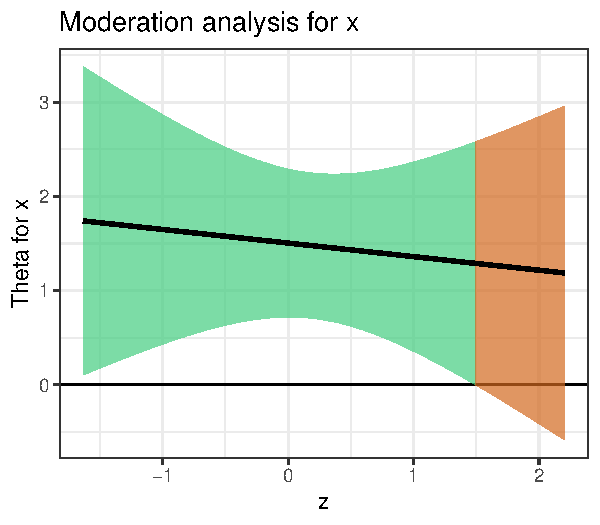
\includegraphics[keepaspectratio]{int3ract_paper_files/figure-pdf/fig-jn2-1.pdf}}

}

\subcaption{\label{fig-jn2-1}Conditional effect of \texttt{x} as a
function of the moderator \texttt{z}.}

\end{minipage}%
%
\begin{minipage}{0.50\linewidth}

\centering{

\pandocbounded{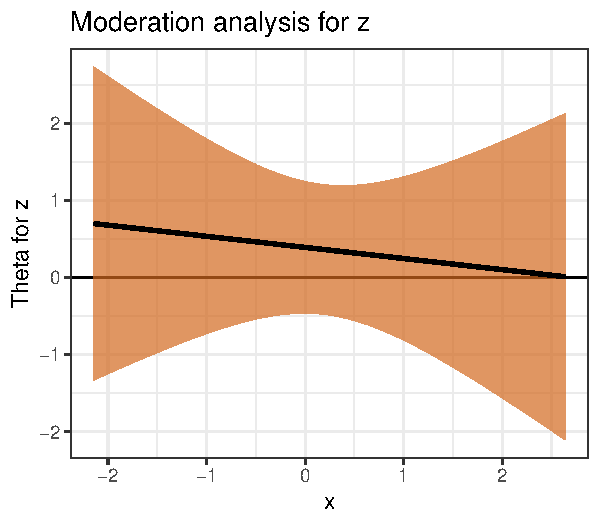
\includegraphics[keepaspectratio]{int3ract_paper_files/figure-pdf/fig-jn2-2.pdf}}

}

\subcaption{\label{fig-jn2-2}Conditional effect of \texttt{z} as a
function of the moderator \texttt{x}.}

\end{minipage}%

\caption{\label{fig-jn2}Johnson--Neyman plots for the two-way
interaction between \texttt{x} and \texttt{z} (\(\alpha = 0.05\)). The
ribbon shows pointwise 95\% confidence bands for the conditional effect;
green shading indicates regions where the effect is statistically
significant, chocolate where it is not.}

\end{figure}%

The returned list \texttt{jn2} contains \texttt{\$param\_table}, a list
of two data frames (one per each variable involved in the interactions)
with columns for the moderator values (\texttt{mod\_vals}), conditional
parameter, its standard error, and \(p\)-value (\texttt{theta\_vals},
\texttt{theta\_se}, and \texttt{theta\_p}), and a logical whether it is
significant given the chosen \texttt{threshold}; and \texttt{\$plots}, a
list of two \textbf{ggplot2} objects.

In each plot the ribbon is filled with \texttt{sig\_color} (default
\texttt{\textquotesingle{}seagreen3\textquotesingle{}}) where
\(|z| > z_{\alpha/2}\) and with \texttt{non\_sig\_color} (default
\texttt{\textquotesingle{}chocolate\textquotesingle{}}) elsewhere.

\subsection{\texorpdfstring{Three-Way Interaction with
\texttt{lm}}{Three-Way Interaction with lm}}\label{three-way-interaction-with-lm}

\begin{Shaded}
\begin{Highlighting}[]
\NormalTok{mod3 }\OtherTok{\textless{}{-}} \FunctionTok{lm}\NormalTok{(y }\SpecialCharTok{\textasciitilde{}}\NormalTok{ x }\SpecialCharTok{*}\NormalTok{ z }\SpecialCharTok{*}\NormalTok{ w, }\AttributeTok{data =}\NormalTok{ dat)}

\NormalTok{jn3 }\OtherTok{\textless{}{-}} \FunctionTok{JNK\_lm}\NormalTok{(mod3,}
               \AttributeTok{theta\_1    =} \StringTok{"x"}\NormalTok{,}
               \AttributeTok{theta\_2    =} \StringTok{"z"}\NormalTok{,}
               \AttributeTok{theta\_3    =} \StringTok{"w"}\NormalTok{,}
               \AttributeTok{range\_size =} \DecValTok{50}\NormalTok{)}
\end{Highlighting}
\end{Shaded}

\begin{figure}[H]

\begin{minipage}{0.50\linewidth}

\centering{

\pandocbounded{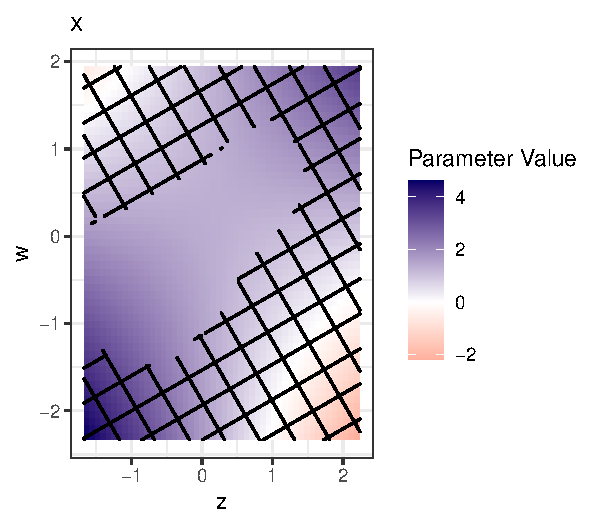
\includegraphics[keepaspectratio]{int3ract_paper_files/figure-pdf/fig-jn3-1.pdf}}

}

\subcaption{\label{fig-jn3-1}Conditional effect of \texttt{x} across the
(\texttt{z}, \texttt{w}) moderator grid.}

\end{minipage}%
%
\begin{minipage}{0.50\linewidth}

\centering{

\pandocbounded{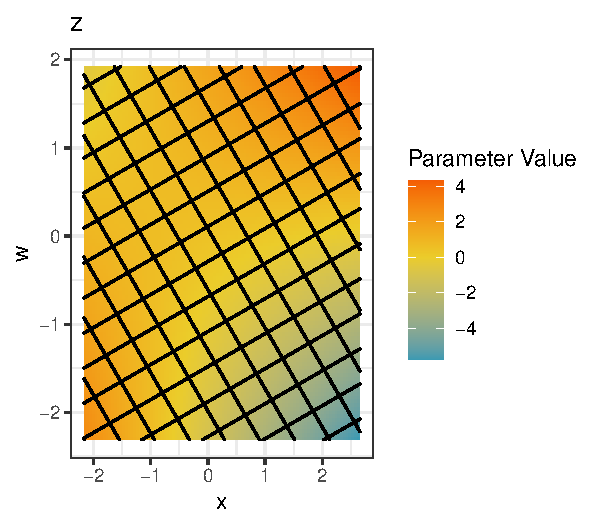
\includegraphics[keepaspectratio]{int3ract_paper_files/figure-pdf/fig-jn3-2.pdf}}

}

\subcaption{\label{fig-jn3-2}Conditional effect of \texttt{z} across the
(\texttt{x}, \texttt{w}) moderator grid.}

\end{minipage}%
\newline
\begin{minipage}{\linewidth}

\centering{

\pandocbounded{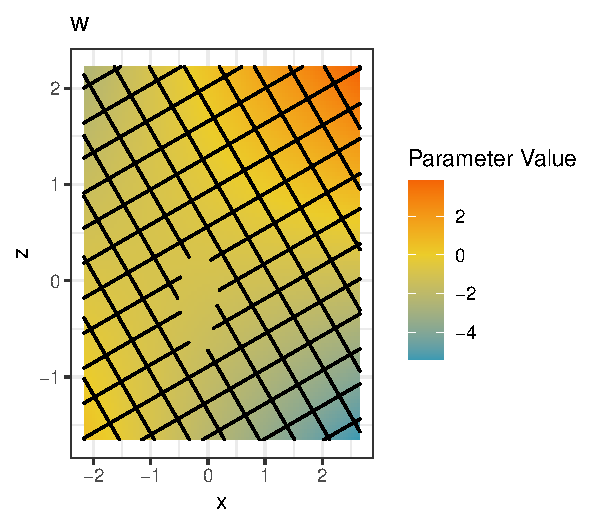
\includegraphics[keepaspectratio]{int3ract_paper_files/figure-pdf/fig-jn3-3.pdf}}

}

\subcaption{\label{fig-jn3-3}Conditional effect of \texttt{w} across the
(\texttt{x}, \texttt{z}) moderator grid.}

\end{minipage}%

\caption{\label{fig-jn3}Johnson--Neyman--Krause heatmaps for the
three-way interaction among \texttt{x}, \texttt{z}, and \texttt{w}
(\texttt{range\_size\ =\ 50}, \(\alpha = 0.05\)). Each cell shows the
conditional point estimate of the focal effect across the
two-dimensional moderator grid; the diverging colour scale runs from red
(negative) through white (zero) to dark blue (positive). Crosshatched
cells indicate regions where the conditional effect is not statistically
significant.}

\end{figure}%

Setting \texttt{range\_size\ =\ 50} produces a \(50 \times 50\) grid for
each of the three heatmaps (i.e., \(3 \times 2{,}500\) conditional
effect evaluations). When all three moderator ranges contain fewer than
eight distinct values, the point estimate is printed in each cell;
otherwise only the colour gradient communicates the magnitude. The
ranges for each variable are by default extracted from the
\texttt{lm}/\texttt{glm} object but need to be supplied explicitly to
\texttt{freq\_int()} or explicitly (see the code chunk below for
\texttt{JNK\_siena()}).

\subsection{\texorpdfstring{Stochastic Actor-Oriented Models
(\texttt{JNK\_siena()})}{Stochastic Actor-Oriented Models (JNK\_siena())}}\label{stochastic-actor-oriented-models-jnk_siena}

SAOMs estimated by \textbf{RSiena}'s \texttt{siena()} (formerly
\texttt{siena07()}) are the primary application domain for which this
package was developed, because interaction effects between network
statistics and actor attributes are common yet difficult to interpret
(T. A. B. Snijders et al. 2026). The interface mirrors
\texttt{JNK\_lm()} but uses integer indices referencing the position of
each effect in the \textbf{RSiena} effects object.

\begin{Shaded}
\begin{Highlighting}[]
\CommentTok{\# Two{-}way interaction}
\NormalTok{x2 }\OtherTok{\textless{}{-}} \FunctionTok{JNK\_siena}\NormalTok{(res,}
                 \AttributeTok{theta\_1      =} \DecValTok{6}\NormalTok{,}
                 \AttributeTok{theta\_2      =} \DecValTok{7}\NormalTok{,}
                 \AttributeTok{theta\_int\_12 =} \DecValTok{8}\NormalTok{,}
                 \AttributeTok{theta\_1vals  =} \SpecialCharTok{{-}}\DecValTok{10}\SpecialCharTok{:}\DecValTok{10}\NormalTok{,}
                 \AttributeTok{theta\_2vals  =} \SpecialCharTok{{-}}\DecValTok{10}\SpecialCharTok{:}\DecValTok{10}\NormalTok{)}

\CommentTok{\# Three{-}way extension}
\NormalTok{x3 }\OtherTok{\textless{}{-}} \FunctionTok{JNK\_siena}\NormalTok{(res,}
                 \AttributeTok{theta\_1       =} \DecValTok{6}\NormalTok{,}
                 \AttributeTok{theta\_2       =} \DecValTok{7}\NormalTok{,}
                 \AttributeTok{theta\_3       =} \DecValTok{5}\NormalTok{,}
                 \AttributeTok{theta\_int\_12  =} \DecValTok{8}\NormalTok{,}
                 \AttributeTok{theta\_int\_13  =} \DecValTok{10}\NormalTok{,}
                 \AttributeTok{theta\_int\_23  =} \DecValTok{9}\NormalTok{,}
                 \AttributeTok{theta\_int\_123 =} \DecValTok{11}\NormalTok{,}
                 \AttributeTok{theta\_1vals   =} \SpecialCharTok{{-}}\DecValTok{10}\SpecialCharTok{:}\DecValTok{10}\NormalTok{,}
                 \AttributeTok{theta\_2vals   =} \SpecialCharTok{{-}}\DecValTok{10}\SpecialCharTok{:}\DecValTok{10}\NormalTok{,}
                 \AttributeTok{theta\_3vals   =} \DecValTok{0}\SpecialCharTok{:}\DecValTok{6}\NormalTok{,}
                 \AttributeTok{range\_size    =} \DecValTok{10}\NormalTok{)}
\end{Highlighting}
\end{Shaded}

The moderator value ranges (\texttt{theta\_1vals},
\texttt{theta\_2vals}, \texttt{theta\_3vals}) should reflect the
empirical support of the corresponding change statistics. By default
\texttt{range\_size\ =\ 500} equidistant points are drawn from these
ranges. The returned tables and plots are named as derived from the
model using the `name' column in the \textbf{RSiena} effects object.

\subsection{\texorpdfstring{Direct Use of
\texttt{freq\_int()}}{Direct Use of freq\_int()}}\label{direct-use-of-freq_int}

Because \texttt{freq\_int()} requires only a coefficient vector and a
covariance matrix, it is straightforward to apply it to models not
covered by the existing wrappers. For instance, for a mixed-effects
model fitted with \textbf{lme4}:

\begin{Shaded}
\begin{Highlighting}[]
\FunctionTok{library}\NormalTok{(lme4)}
\FunctionTok{library}\NormalTok{(int3ract)}

\NormalTok{lme\_mod }\OtherTok{\textless{}{-}} \FunctionTok{lmer}\NormalTok{(y }\SpecialCharTok{\textasciitilde{}}\NormalTok{ x }\SpecialCharTok{*}\NormalTok{ z }\SpecialCharTok{+}\NormalTok{ (}\DecValTok{1} \SpecialCharTok{|}\NormalTok{ group), }\AttributeTok{data =}\NormalTok{ dat)}

\NormalTok{all\_coef }\OtherTok{\textless{}{-}} \FunctionTok{fixef}\NormalTok{(lme\_mod)}
\NormalTok{all\_vcov }\OtherTok{\textless{}{-}} \FunctionTok{as.matrix}\NormalTok{(}\FunctionTok{vcov}\NormalTok{(lme\_mod))}
\NormalTok{sel      }\OtherTok{\textless{}{-}} \FunctionTok{c}\NormalTok{(}\StringTok{"x"}\NormalTok{, }\StringTok{"z"}\NormalTok{, }\StringTok{"x:z"}\NormalTok{)}

\FunctionTok{freq\_int}\NormalTok{(}\AttributeTok{name  =} \FunctionTok{c}\NormalTok{(}\StringTok{"x"}\NormalTok{, }\StringTok{"z"}\NormalTok{),}
         \AttributeTok{coefs =}\NormalTok{ all\_coef[sel],}
         \AttributeTok{covar =}\NormalTok{ all\_vcov[sel, sel],}
         \AttributeTok{vals  =} \FunctionTok{list}\NormalTok{(}\FunctionTok{range}\NormalTok{(dat}\SpecialCharTok{$}\NormalTok{x), }\FunctionTok{range}\NormalTok{(dat}\SpecialCharTok{$}\NormalTok{z)),}
         \AttributeTok{range\_size =} \DecValTok{1000}\NormalTok{)}
\end{Highlighting}
\end{Shaded}

The same pattern applies to survival models (\textbf{survival}), ordinal
regression (\textbf{MASS}), beta regression (\textbf{betareg}), and any
other estimation that that provides parameter estimates and their
covariances.

\section{\texorpdfstring{Bayesian Usage:
\texttt{JNSienaBayes()}}{Bayesian Usage: JNSienaBayes()}}\label{sec-bayes}

For multi-group Bayesian SAOMs estimated with \textbf{multiSiena} (T.
Snijders, Koskinen, and Ripley 2026; Koskinen and Snijders 2023), the
full posterior distribution over model parameters replaces the class
JN-framework. The function \texttt{JNSienaBayes()} automatically detects
whether each required parameter has been estimated as a fixed effect
(\(\mu\); shared across groups) or as a random effect (\(\eta\);
group-varying, with a hyper-parameter), and extracts the appropriate
posterior draws.

\begin{Shaded}
\begin{Highlighting}[]
\NormalTok{jnb2 }\OtherTok{\textless{}{-}} \FunctionTok{JNSienaBayes}\NormalTok{(}\AttributeTok{sbo          =}\NormalTok{ my\_multiSiena\_result,}
                     \AttributeTok{theta\_1      =} \DecValTok{4}\NormalTok{,}
                     \AttributeTok{theta\_2      =} \DecValTok{7}\NormalTok{,}
                     \AttributeTok{theta\_int\_12 =} \DecValTok{9}\NormalTok{,}
                     \AttributeTok{theta\_1\_vals =} \FunctionTok{c}\NormalTok{(}\SpecialCharTok{{-}}\DecValTok{1}\NormalTok{,}\DecValTok{0}\NormalTok{,}\DecValTok{1}\NormalTok{),}
                     \AttributeTok{theta\_2\_vals =} \FunctionTok{seq}\NormalTok{(}\SpecialCharTok{{-}}\DecValTok{3}\NormalTok{,}\DecValTok{3}\NormalTok{,}\FloatTok{0.5}\NormalTok{),}
                     \AttributeTok{burnIn       =} \DecValTok{500}\NormalTok{,}
                     \AttributeTok{thin         =} \DecValTok{2}\NormalTok{,}
                     \AttributeTok{save         =} \ConstantTok{FALSE}\NormalTok{)}
\end{Highlighting}
\end{Shaded}

\begin{figure}[H]

\begin{minipage}{\linewidth}

\centering{

\pandocbounded{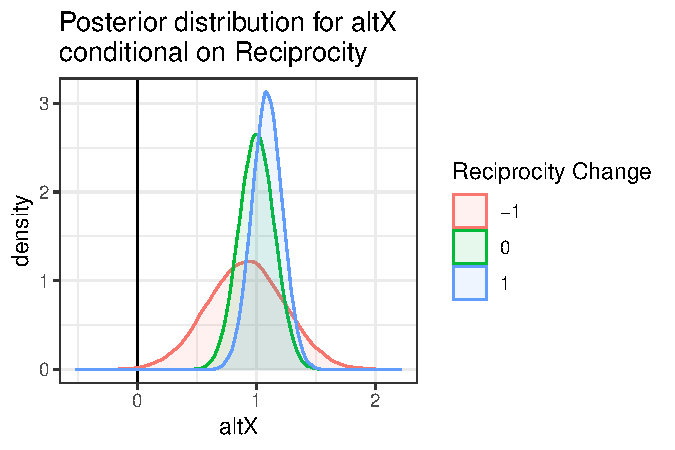
\includegraphics[keepaspectratio]{int3ract_paper_files/figure-pdf/fig-bayes-2fake-1.pdf}}

}

\subcaption{\label{fig-bayes-2fake-1}Posterior densities for altX
conditional on simultaneous changes in reciprocity. In this example,
altX is always positive but has larger variance when reciprocity would
decrease (i.e., a reciprocal tie to someone with negative values on the
covariate would be broken, leading to -1 in recirpocity but overall an
increase in altX).}

\end{minipage}%
\newline
\begin{minipage}{\linewidth}

\centering{

\pandocbounded{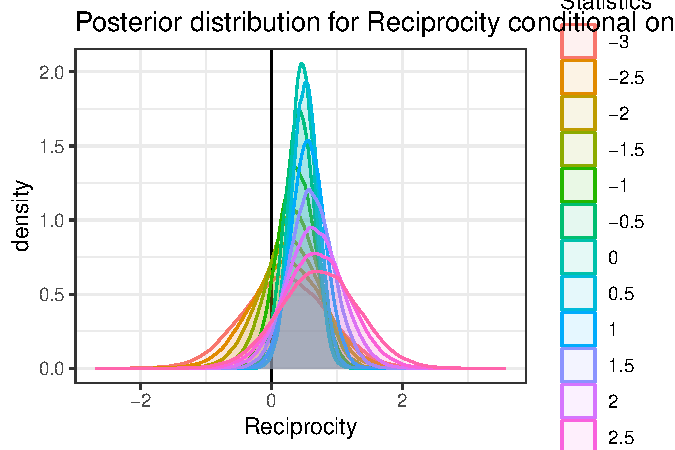
\includegraphics[keepaspectratio]{int3ract_paper_files/figure-pdf/fig-bayes-2fake-2.pdf}}

}

\subcaption{\label{fig-bayes-2fake-2}Posterior densities for reciprocity
conditional on simultaneous changes in altX. Here, while generally
positive, reciprocity only has a consistently positive effect on tie
formation when altX changes moderately, around -1 to 1 (curves with low
color saturation). While reciprocity gets more positive with increasing
values in the change of altX, the posterior variance increases as well.}

\end{minipage}%

\caption{\label{fig-bayes-2fake}Conditional posterior densities for the
parameters for reciprocity and altX on a attribute.}

\end{figure}%

The returned object is a named list similar to those returned for
frequentist interactions. Each table here contains the posterior mean,
posterior SD, Bayesian \(p\)-value
(\(\Pr(\tilde{\theta}_X > 0 \mid \text{data}, \text{model}, \text{prior})\)),
and 2.5th and 97.5th percentiles of the conditional posterior for each
moderator value.

When \texttt{hyper\_only\ =\ FALSE} and at least one of the involved
parameters is randomly varying between groups, \texttt{JNSienaBayes()}
additionally loops over all \(G\) groups and produces group-specific
plots and tables, returned under the key
\texttt{random\_groups\_effects}. This is useful for assessing
heterogeneity of interaction effects across networks. Two additional
arguments are helpful when many plots are made: \texttt{save\ =\ TRUE}
will save each plot with \texttt{ggsave()}. To avoid cluttering your
working directory, \texttt{folder} provides the location of a folder
where the plots will be stored. If no input is provided, a new folder
\texttt{int3ract\ JNplots} will be created (note that RStudio will ask
you in the console whether such a folder is allowed to be created, if it
does not exist yet).

For three-way interactions, the call is extended as usual. The
\texttt{thresholds} argument (a vector of length 2, e.g.,
\texttt{c(0.05,\ 0.95)}) determines which cells of the posterior-mean
heatmap are crosshatched: cells whose Bayesian \(p\)-value falls inside
the interval \([\mathrm{threshold}_1, \mathrm{threshold}_2]\) are
treated as non-significant.

\begin{Shaded}
\begin{Highlighting}[]
\NormalTok{jnb3 }\OtherTok{\textless{}{-}} \FunctionTok{JNSienaBayes}\NormalTok{(}\AttributeTok{sbo           =}\NormalTok{ my\_multiSiena\_result,}
                     \AttributeTok{theta\_1       =} \DecValTok{4}\NormalTok{,}
                     \AttributeTok{theta\_2       =} \DecValTok{10}\NormalTok{,}
                     \AttributeTok{theta\_3       =} \DecValTok{9}\NormalTok{,}
                     \AttributeTok{theta\_int\_12  =} \DecValTok{21}\NormalTok{,}
                     \AttributeTok{theta\_int\_13  =} \DecValTok{22}\NormalTok{,}
                     \AttributeTok{theta\_int\_23  =} \DecValTok{11}\NormalTok{,}
                     \AttributeTok{theta\_int\_123 =} \DecValTok{23}\NormalTok{,}
                     \AttributeTok{theta\_1\_vals  =} \FunctionTok{seq}\NormalTok{(}\SpecialCharTok{{-}}\DecValTok{2}\NormalTok{, }\DecValTok{2}\NormalTok{, }\AttributeTok{length.out =} \DecValTok{50}\NormalTok{),}
                     \AttributeTok{theta\_2\_vals  =} \FunctionTok{seq}\NormalTok{(}\SpecialCharTok{{-}}\DecValTok{2}\NormalTok{, }\DecValTok{2}\NormalTok{, }\AttributeTok{length.out =} \DecValTok{50}\NormalTok{),}
                     \AttributeTok{theta\_3\_vals  =} \FunctionTok{seq}\NormalTok{(}\SpecialCharTok{{-}}\DecValTok{2}\NormalTok{, }\DecValTok{2}\NormalTok{, }\AttributeTok{length.out =} \DecValTok{50}\NormalTok{),}
                     \AttributeTok{thresholds    =} \FunctionTok{c}\NormalTok{(}\FloatTok{0.05}\NormalTok{, }\FloatTok{0.95}\NormalTok{),}
                     \AttributeTok{burnIn        =} \DecValTok{500}\NormalTok{,}
                     \AttributeTok{thin          =} \DecValTok{2}\NormalTok{)}
\end{Highlighting}
\end{Shaded}

\begin{figure}[H]

\begin{minipage}{\linewidth}

\centering{

\pandocbounded{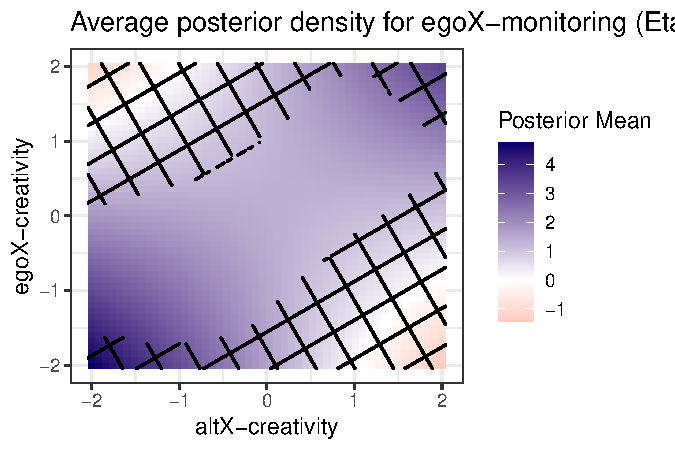
\includegraphics[keepaspectratio]{int3ract_paper_files/figure-pdf/fig-bayes-3fake-1.pdf}}

}

\subcaption{\label{fig-bayes-3fake}Mean posterior densities for the
effect of ego's self-monitoring on tie creation conditional on ego's and
alter's creativity. In this example, self-monitoring has a positive
effect on tie creation when both ego and alter have similar levels of
creativity.}

\end{minipage}%

\caption{\label{fig-bayes-3fake}Figures for Bayesian 3-way interactions}

\end{figure}%

\section{Graphical Output and Customisation}\label{sec-graphics}

All plots are standard \textbf{ggplot2} objects (Wickham 2016) and can
be further modified using \textbf{ggplot2}'s layer system. The
crosshatch pattern for non-significant regions is produced by
\textbf{ggpattern} (Stewart 2022). Table~\ref{tbl-colors} documents the
colour and pattern parameters shared across all plotting functions.

\begin{table}

\caption{\label{tbl-colors}Colour and pattern parameters available in
all \textbf{int3ract} plotting functions. Default colour values are
highlighted in their respective colour.}

\centering{

\fontsize{12.0pt}{14.0pt}\selectfont
\begin{tabular*}{\linewidth}{@{\extracolsep{\fill}}>{\raggedright\arraybackslash}p{\dimexpr 120.00pt -2\tabcolsep-1.5\arrayrulewidth}>{\raggedright\arraybackslash}p{\dimexpr 247.50pt -2\tabcolsep-1.5\arrayrulewidth}>{\raggedright\arraybackslash}p{\dimexpr 82.50pt -2\tabcolsep-1.5\arrayrulewidth}}
\toprule
{\small Parameter} & Description & {\small Default} \\ 
\midrule\addlinespace[2.5pt]
{\small sig\_color} & Ribbon fill for significant regions (2-way) & {\small \cellcolor[HTML]{43CD80}{\textcolor[HTML]{000000}{`seagreen3'}}} \\ 
{\small non\_sig\_color} & Ribbon fill for non-significant regions (2-way) & {\small \cellcolor[HTML]{D2691E}{\textcolor[HTML]{FFFFFF}{`chocolate'}}} \\ 
{\small line\_color} & Point-estimate line colour (2-way) & {\small \cellcolor[HTML]{000000}{\textcolor[HTML]{FFFFFF}{`black'}}} \\ 
{\small color\_low} & Low end of diverging fill scale (heatmaps) & {\small \cellcolor[HTML]{F05039}{\textcolor[HTML]{FFFFFF}{`\#F05039'}}} \\ 
{\small color\_mid} & Midpoint colour of diverging fill scale & {\small \cellcolor[HTML]{FFFFFF}{\textcolor[HTML]{000000}{`white'}}} \\ 
{\small color\_high} & High end of diverging fill scale & {\small \cellcolor[HTML]{000066}{\textcolor[HTML]{FFFFFF}{`\#000066'}}} \\ 
{\small color\_grid} & Crosshatch line colour & {\small \cellcolor[HTML]{000000}{\textcolor[HTML]{FFFFFF}{`black'}}} \\ 
{\small grid\_density} & Density of crosshatch lines & {\small 0.01} \\ 
{\small grid\_spacing} & Spacing between crosshatch lines & {\small 0.1} \\ 
{\small color\_values} & Within-cell text colour (heatmaps, ≤ 7 values) & {\small \cellcolor[HTML]{666666}{\textcolor[HTML]{FFFFFF}{`grey40'}}} \\ 
{\small crosshatch\_non\_sig} & If TRUE, crosshatch marks the non-significant region & {\small TRUE} \\ 
\bottomrule
\end{tabular*}

}

\end{table}%

\section{Summary and Outlook}\label{sec-conc}

\textbf{int3ract} provides a unified interface for the Johnson--Neyman
technique and its three-way extension across a broad class of
frequentist and Bayesian models. By exposing the core computation in a
single model-agnostic function, \texttt{freq\_int()}, the package
invites adoption beyond the two model classes for which dedicated
wrappers currently exist. Future development plans include:

\begin{enumerate}
\def\labelenumi{\arabic{enumi}.}
\tightlist
\item
  A wrapper for \texttt{merMod} objects from \textbf{lme4} to allow for
  randomly varying interactions.
\item
  A consideration for FDR-correction.
\item
  A general Bayesian application
\end{enumerate}

Researchers are encouraged to report not only the JN boundaries but also
the full plots as supplementary material, in keeping with calls for more
transparent and complete reporting of interaction effects (Simonsohn,
Simmons, and Nelson 2020).

\section{Dependencies}\label{dependencies}

To give due credit, next to the already listed packages,
\textbf{int3ract} also depends on \textbf{scales},\textbf{tidyr},
\textbf{tibble} Müller and Wickham (2026).

\section*{References}\label{references}
\addcontentsline{toc}{section}{References}

\phantomsection\label{refs}
\begin{CSLReferences}{1}{0}
\bibitem[\citeproctext]{ref-Bauer2005}
Bauer, Daniel J., and Patrick J. Curran. 2005. {``Probing Interactions
in Fixed and Multilevel Regression: Inferential and Graphical
Techniques.''} \emph{Multivariate Behavioral Research} 40 (3): 373--400.
\url{https://doi.org/10.1207/s15327906mbr4003_5}.

\bibitem[\citeproctext]{ref-Johnson1936}
Johnson, Palmer O., and Jerzy Neyman. 1936. {``Tests of Certain Linear
Hypotheses and Their Applications to Some Educational Problems.''}
\emph{Statistical Research Memoirs} 1: 57--93.

\bibitem[\citeproctext]{ref-Kosk23}
Koskinen, Johan H., and Tom A. B. Snijders. 2023. {``Multilevel
Longitudinal Analysis of Social Networks.''} \emph{Journal of the Royal
Statistical Society, Series A} 186: 376--400.

\bibitem[\citeproctext]{ref-Long2019}
Long, Jacob Scott. 2019. \emph{{interactions}: Comprehensive,
User-Friendly Toolkit for Probing Interactions}.
\url{https://cran.r-project.org/package=interactions}.

\bibitem[\citeproctext]{ref-Long2020}
---------. 2020. \emph{{jtools}: Analysis and Presentation of Social
Scientific Data}. \url{https://cran.r-project.org/package=jtools}.

\bibitem[\citeproctext]{ref-tibble}
Müller, Kirill, and Hadley Wickham. 2026. \emph{Tibble: Simple Data
Frames}. \url{https://doi.org/10.32614/CRAN.package.tibble}.

\bibitem[\citeproctext]{ref-Potthoff1964}
Potthoff, Richard F. 1964. {``On the {Johnson--Neyman} Technique and
Some Extensions Thereof.''} \emph{Psychometrika} 29 (3): 241--56.
\url{https://doi.org/10.1007/BF02289721}.

\bibitem[\citeproctext]{ref-Preacher2006}
Preacher, Kristopher J., Patrick J. Curran, and Daniel J. Bauer. 2006.
{``Computational Tools for Probing Interactions in Multiple Linear
Regression, Multilevel Modeling, and Latent Curve Analysis.''}
\emph{Journal of Educational and Behavioral Statistics} 31 (4): 437--48.
\url{https://doi.org/10.3102/10769986031004437}.

\bibitem[\citeproctext]{ref-Simonsohn2020}
Simonsohn, Uri, Joseph P. Simmons, and Leif D. Nelson. 2020.
{``Specification Curve Analysis.''} \emph{Nature Human Behaviour} 4
(11): 1208--14. \url{https://doi.org/10.1038/s41562-020-0912-z}.

\bibitem[\citeproctext]{ref-Snijders26}
Snijders, Tom A. B., Ruth M. Ripley, Krists Boitmanis, Christian
Steglich, Nynke M. D. Niezink, Viviana Amati, and Felix Schoenenberger.
2026. \emph{Siena - Simulation Investigation for Empirical Network
Analysis}. Groningen, The Netherlands: University of Groningen.
\url{https://www.stats.ox.ac.uk/~snijders/siena/}.

\bibitem[\citeproctext]{ref-SienaMult}
Snijders, Tom, Johan Koskinen, and Ruth Ripley. 2026. \emph{multiSiena -
Simulation Investigation for Multilevel Empirical Network Analysis}.
Groningen, The Netherlands: University of Groningen.
\url{http://www.stats.ox.ac.uk/~snijders/siena}.

\bibitem[\citeproctext]{ref-ggpattern2022}
Stewart, Mike. 2022. \emph{{ggpattern}: {ggplot2} Pattern Geoms}.
\url{https://cran.r-project.org/package=ggpattern}.

\bibitem[\citeproctext]{ref-Wickham2016}
Wickham, Hadley. 2016. \emph{{ggplot2}: Elegant Graphics for Data
Analysis}. New York: Springer-Verlag.
\url{https://doi.org/10.1007/978-3-319-24277-4}.

\bibitem[\citeproctext]{ref-scales}
Wickham, Hadley, Thomas Lin Pedersen, and Dana Seidel. 2025.
\emph{Scales: Scale Functions for Visualization}.
\url{https://doi.org/10.32614/CRAN.package.scales}.

\bibitem[\citeproctext]{ref-tidy}
Wickham, Hadley, Davis Vaughan, and Maximilian Girlich. 2025.
\emph{Tidyr: Tidy Messy Data}.
\url{https://doi.org/10.32614/CRAN.package.tidyr}.

\end{CSLReferences}




\end{document}
